\documentclass[../main/thesis.tex]{subfiles}
\graphicspath{{/home/arefk/uio/MScThesis_AreKvanum2022_SeaIceML/thesis/performance_assessment/figures/}}
\begin{document}

\section{Model performance}
The following section intends to explore the performance and capabilities of the deep learning system. Where the previous section \ref{sec:model_development_results} assessed the intra-training model performance, the current section will compare a benchmark deep learning model against baselines and physical models. The physical models have been previously described in section \ref{sec:datasets}, and the baselines (although previously mentioned and to some extent utilized) will be derived in the following subsection. This section will first assess model performance against persistence. Afterwards, the deep learning system will be compared against other physical models. Setup and considerations will be described as they become relevant.

\subsection{Baselines}
\label{sec:baselines}
To types of baselines are considered, persistence and a linear trend. A persistence forecast is constant in time. Regardless of the forecast lead time the initial values for all grid cells are kept constant. Moreover, the autocorrelation of sea ice concentration from the sea ice charts was shown in section \ref{sec:sea-ice-charts} to be high for short lead times. 

\todo{I discussion nevne at persistence er vanskelig å slå, vise resultater fra \protect\citep{Zampieri2019}}

The second baseline uses the linear trend, as described in section \ref{sec:osisafssmis} and used as predictor for the deep learning system \ref{sec:data_trend}. However, the computed linear trend will be applied pixelwise to advance the initial state forward in time to a given lead time. As the linear trend is computed from OSI SAF ssmis observations, it will consequently be applied to the same dataset. For clarity, the linear trend forecast is computed on the 1km AROME Arctic grid, and the computed values are clipped to match the valid value range, i.e. $\text{values} < 0 \rightarrow \text{values} = 0 \land \text{values} > 100 \rightarrow \text{values} = 100$.


\subsection{Verifying performance against persistence}
For this section, a model representing a benchmark with a depth of 256 channels in the final feature map, learning rate $=0.001$ and all predictor variables have been used. Only the core training dataset was used for training(2019 and 2020).

The seasonal distribution of average ice edge displacement for all sea ice categories found in the sea ice charts are shown for the deep learning system and persistence are displayed in figure \ref{fig:violins}. Figure \ref{fig:violins} demonstrates the predictive performance for the deep learning system measured at each resolved contour. In figure \ref{fig:violins} b), c), d) and e), the deep learning system achieves a lower median 25-th and 75-th percentile than persistence.

\begin{figure}
    \centering
    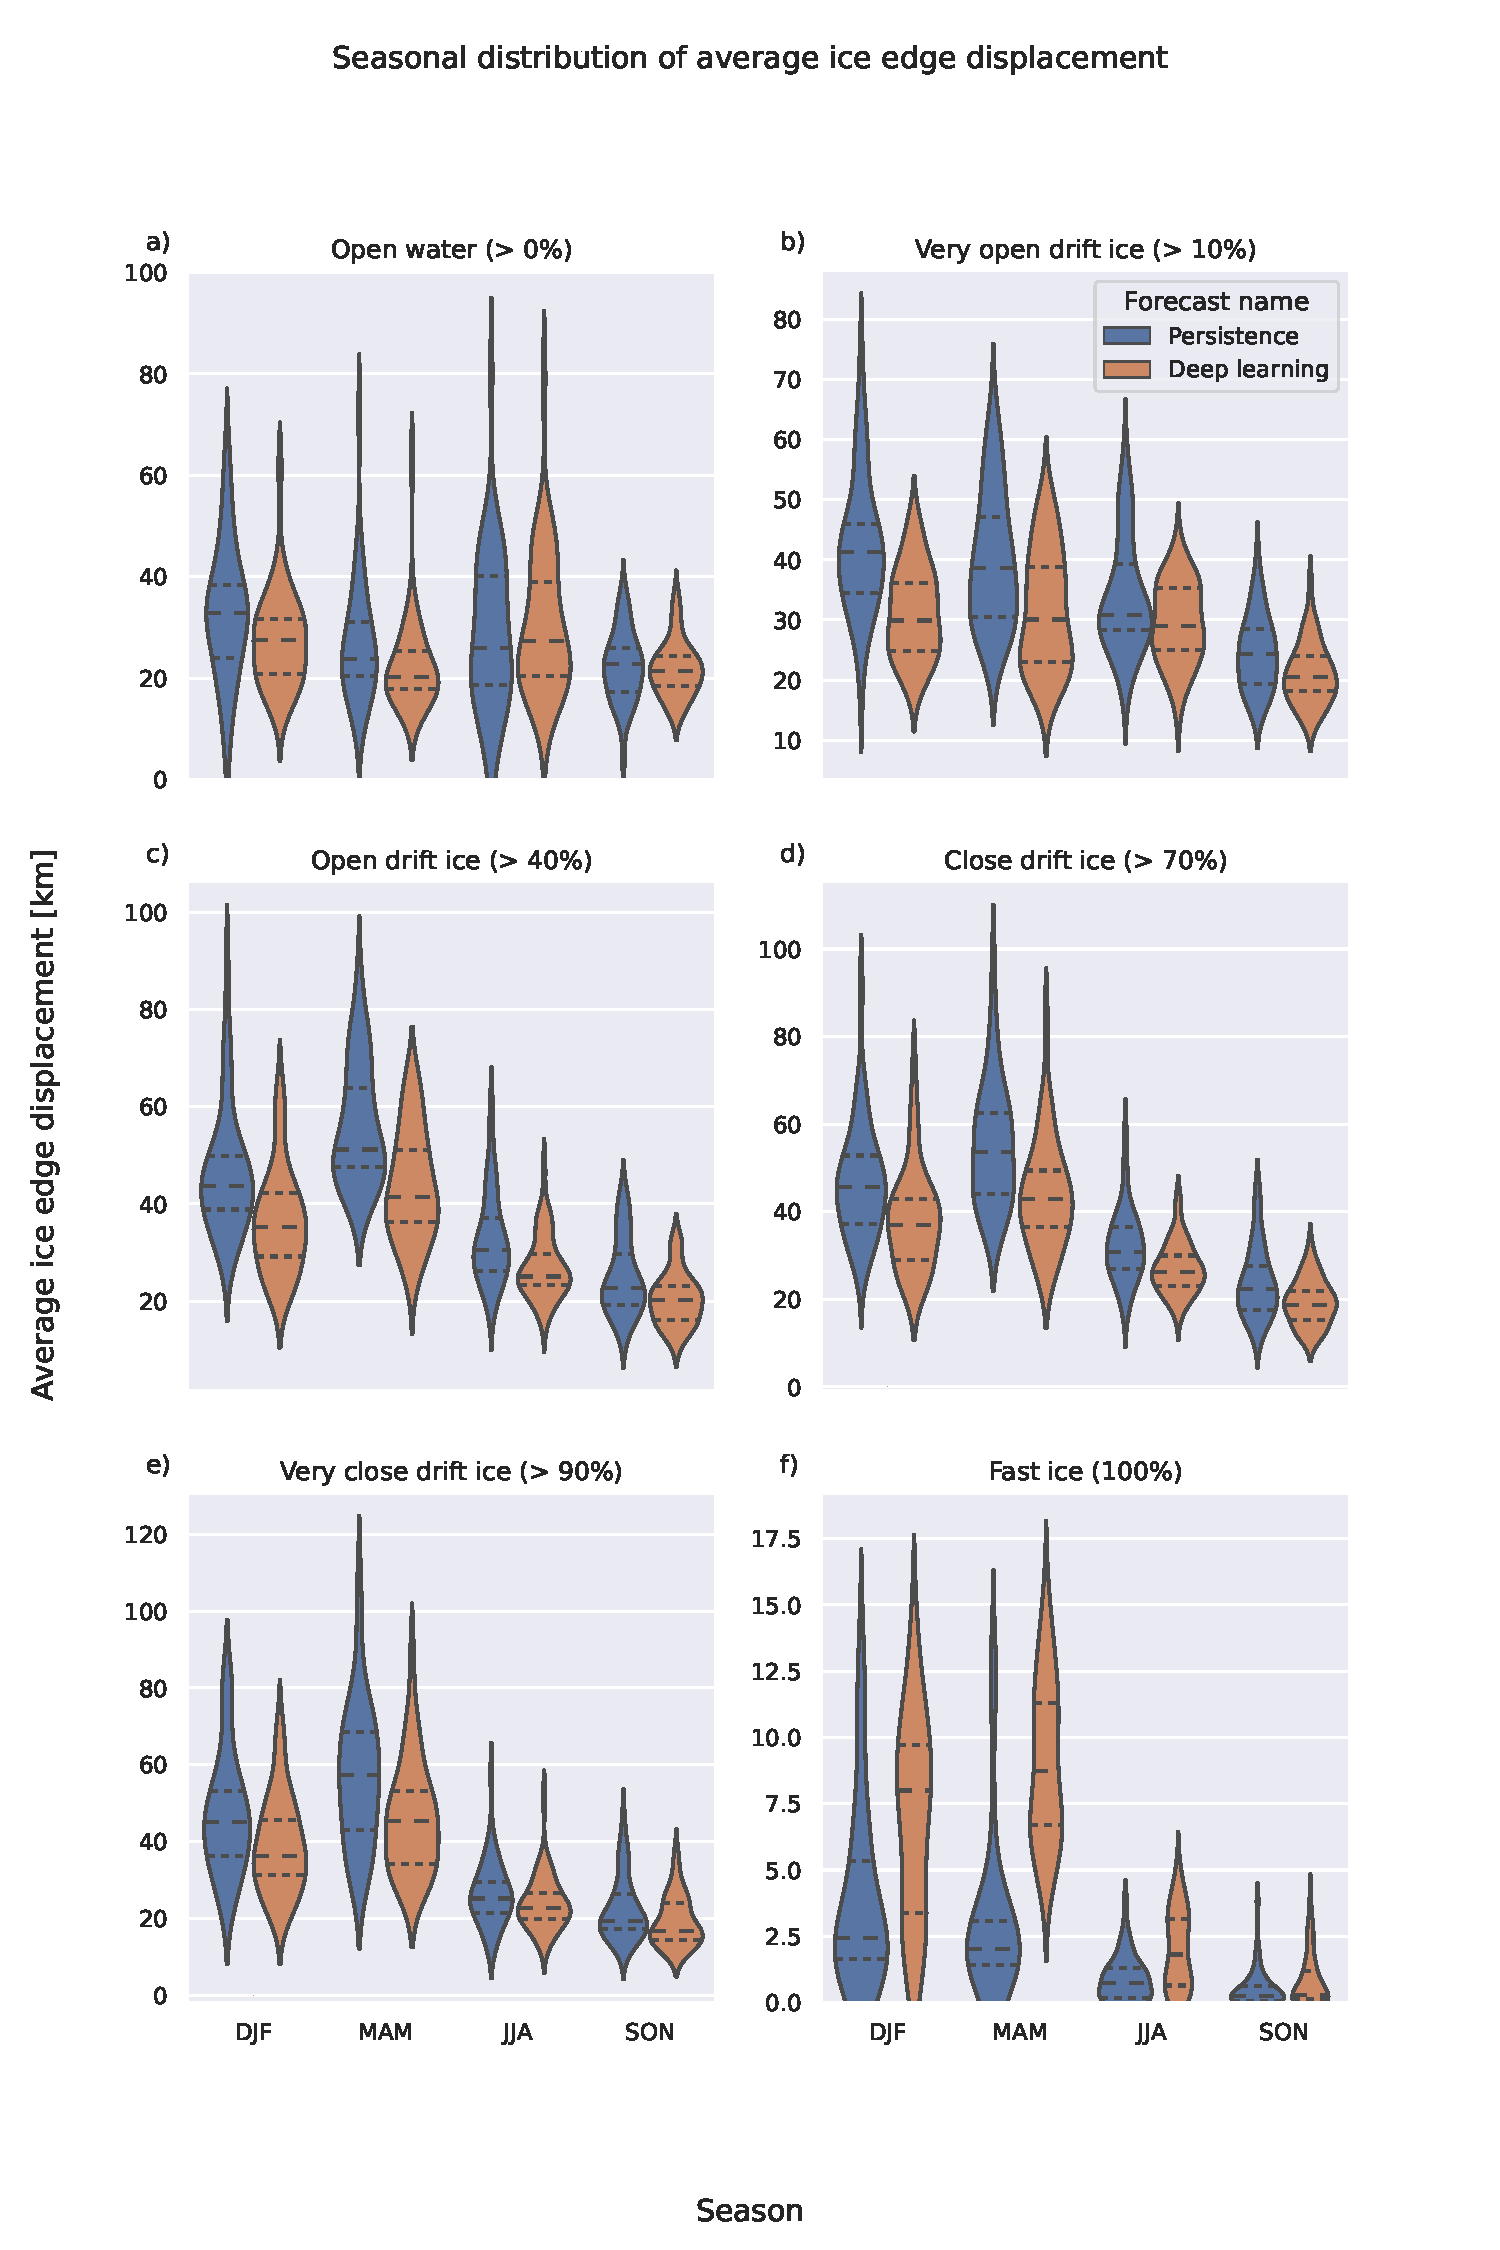
\includegraphics[width=.77\textwidth]{violin_distribution_benchmark}
    \caption{\label{fig:violins}Seasonal distribution of the mean ice edge displacement (Normalized IIEE) for the different sea ice chart categories in the form of cumulative contours. The related sea ice concentration range for each contour is also included. The lower and upper dashed line denote the interquartile range, with the middlemost dashed line showing the distribution median.}
\end{figure}

Figures \ref{fig:mean_annual_confidence} and \ref{fig:confidence_seasonal} shows the model confidence as an annual mean for all output contours (figure \ref{fig:mean_annual_confidence}) and the $(> 10\%)$ contour distributed seasonally (figure \ref{fig:confidence_seasonal}). The confidence values shown are output pixel values after the sigmoid (equation \ref{eq:sigmoid}), such that values closer than 1 are pixels that the model is more confident to belong in the outputted contour. Likewise, values closer to 0 are confident not to belong to the targeted contour.

\begin{figure}
    \centering
    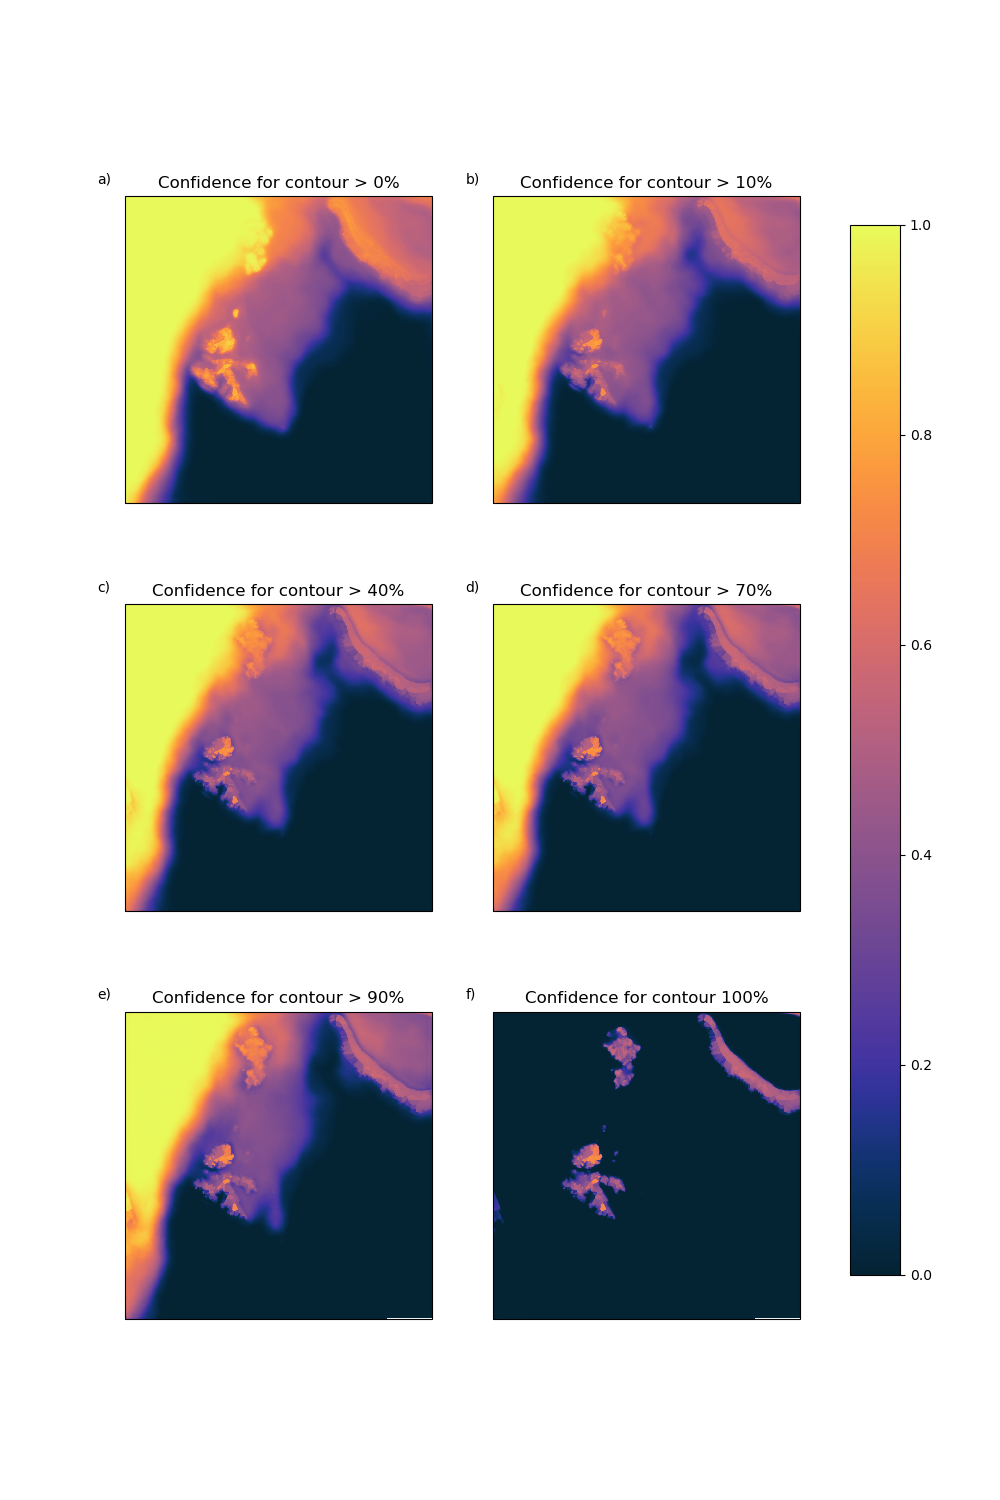
\includegraphics[width=.77\textwidth]{confidence_mean_annual}
    \caption{\label{fig:mean_annual_confidence}Mean annual probabilities for the different cumulative contours outputted by the model (the class ice free open water is not shown).}
\end{figure}

\begin{figure}
    \centering
    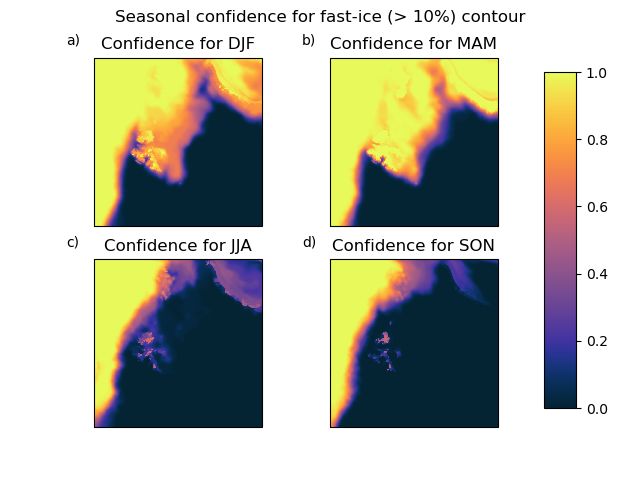
\includegraphics[width=\textwidth]{confidence_test_contour_2}
    \caption{\label{fig:confidence_seasonal}Mean seasonal confidence for the $(> 10\%)$ cumulative contour.}
\end{figure}



\subsection{Inter-product comparison}
This section covers results regarding the multi-product comparison. First, the preparation of samples as well as setup of comparison environment is described. The physical models considered for this comparison are neXtSIM \citep{Williams2021} presented in section \ref{sec:nextsim} and Barents-2.5 \citep{Roehrs2022} presented in section \ref{sec:barents}, whereas the considered baselines are persistence and the linear sea ice concentration trend described in section \ref{sec:baselines}. 

When comparing against multiple products, the coarsest resolution model is used as a common spatial resolution, although all products are interpolated onto the AROME Arctic projection. As both baselines have a daily forecast frequency, comparing either with a deep learning prediction involves identifying the forecast with similar bulletin date and valid date, i.e. initialized at the same day and targeting the same lead time.

Comparing against the two physical models are less intuitive, as both physical models have an hourly forecast frequency \citep{Williams2021, Roehrs2022}. First, given a published sea ice chart, the comparable physical model is initialized the following day at 00:00 UTC. Furthermore, a daily mean is computed from the 24 predictions made by the physical model when it covers the valid date of the deep learning forecast. From this setup, the mean of the first 24 hours of a forecast from a physical model is compared against a deep learning prediction with one day lead time, the mean between 24 and 48 hours are compared against a deep learning prediction with two day lead and the mean of the third predicted day is compared against a deep learning system with three day lead time. Figure \ref{fig:product_compare_timeline} summarizes the process. Note that Barents-2.5 only have a 66 hour lead time \citep{Roehrs2022}, thus the mean between $t = 48$ and $t = 66$ is computed when comparing against a three day lead time prediction.


\begin{figure}
    \centering
    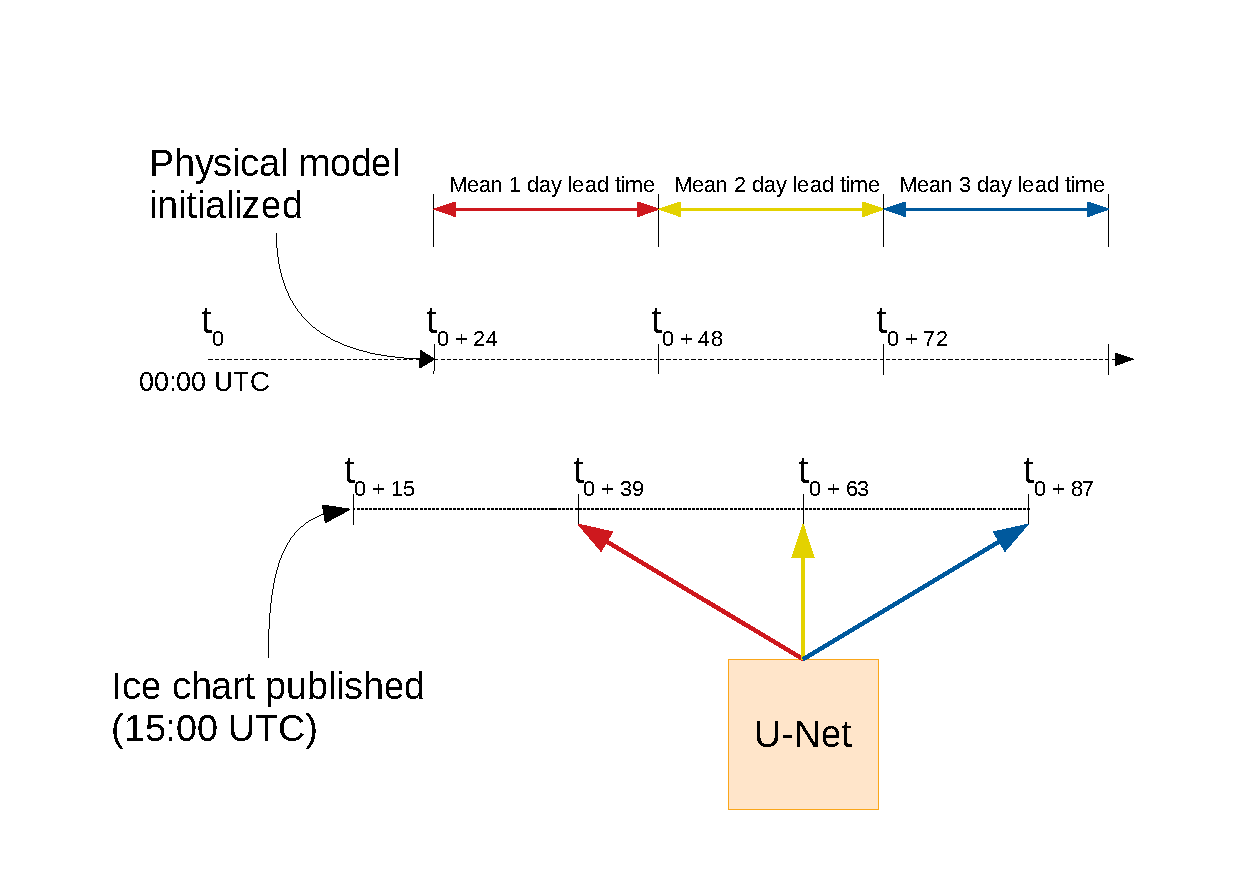
\includegraphics[width=\textwidth]{product_compare_timeline}
    \caption{\label{fig:product_compare_timeline}Overview describing how a physical model with an hourly frequency is compared against a deep learning forecast. Timestamps are hourly, and relative to 00:00 UTC the day a sea ice chart is published. The physical model is initialized the following day. Colors are used to denote comparability, with red $= 1$, yellow $= 2$ and green $= 3$ day lead time. }
\end{figure}


\subsection{Preparing data}
The logic behind sample creation is similar for both physical models. The idea is that the bulletin date of the physical forecasting system is +1 the bulletin date of the machine learning forecast. Furthermore, a daily mean is computed from the forecast based on the lead time of the forecast. I.e., a 1 day lead time for the machine learning forecast would constitute a daily mean of the first 24 hours forecasted by a physical forecasting system starting at 00 the following day of the machine learning bulletin date. 


\biblio
\end{document}